\documentclass[tikz,border=10pt]{standalone}
\usepackage[T1]{fontenc}
\usepackage{tikz}
\usetikzlibrary{arrows.meta, positioning, shapes, calc}

\begin{document}
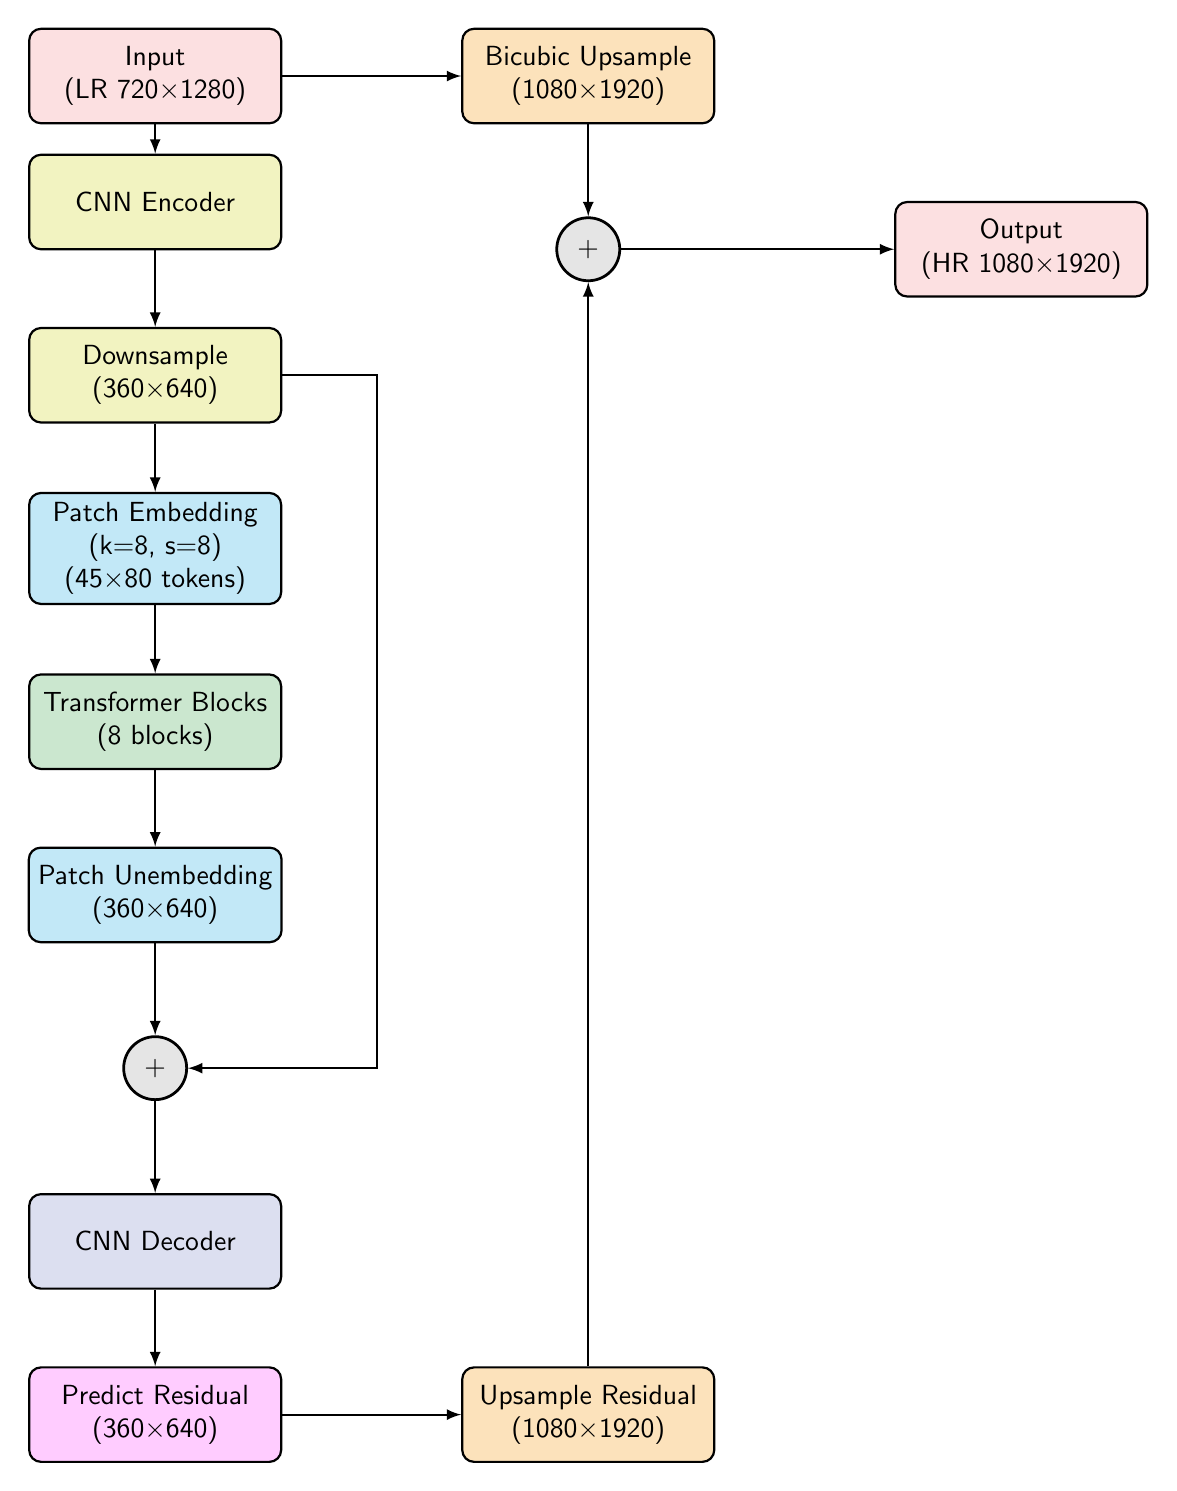
\begin{tikzpicture}[
    font=\sffamily,
    >=latex,                 % Use LaTeX arrowheads
    node distance=2.2cm,     % Default spacing between nodes
    on grid,
    block/.style={
        draw,
        thick,
        rounded corners=0.15cm,
        align=center,
        minimum width=3.2cm,
        minimum height=1.2cm
    }
]

%--- Define colors for blocks ---
\definecolor{colorInput}{RGB}{252,224,225}         % Pink
\definecolor{colorUpsample}{RGB}{252,226,187}      % Light Orange
\definecolor{colorEncoder}{RGB}{242,243,193}       % Light Yellow
\definecolor{colorPatchEmbed}{RGB}{194,232,247}    % Light Blue
\definecolor{colorTransformer}{RGB}{203,231,207}   % Light Green
\definecolor{colorDecoder}{RGB}{220,223,240}       % Light Purple
\definecolor{colorResidual}{RGB}{255,204,255}      % Light Magenta
\definecolor{colorGray}{gray}{0.9}                 % Gray background for sum nodes

%------------------------------------
% LEFT COLUMN: MAIN UPSCALER PIPELINE
%------------------------------------

% 1) Low-res input
\node[block, fill=colorInput] (lr_input)
{Input\\(LR 720$\times$1280)};

% 2) CNN Encoder
\node[block, fill=colorEncoder, below=1.6cm of lr_input] (encoder)
{CNN Encoder};

% 3) Downsample
\node[block, fill=colorEncoder, below=of encoder] (downsample)
{Downsample\\(360$\times$640)};

% 4) Patch Embedding
\node[block, fill=colorPatchEmbed, below=of downsample] (patch_embed)
{Patch Embedding\\(k=8, s=8)\\(45$\times$80 tokens)};

% 5) Transformer
\node[block, fill=colorTransformer, below=of patch_embed] (transformer)
{Transformer Blocks\\(8 blocks)};

% 6) Patch Unembedding
\node[block, fill=colorPatchEmbed, below=of transformer] (patch_unembed)
{Patch Unembedding\\(360$\times$640)};

% Skip-sum node (circle with +) after patch unembedding
\node[draw, circle, line width=1pt, minimum size=0.8cm, fill=colorGray]
(skip_sum)
[below=2.2cm of patch_unembed] {+};

% 7) CNN Decoder
\node[block, fill=colorDecoder, below=2.2cm of skip_sum] (decoder)
{CNN Decoder};

% 8) Predict Residual
\node[block, fill=colorResidual, below=of decoder] (residual)
{Predict Residual\\(360$\times$640)};


%------------------------------------
% CENTER COLUMN: GLOBAL RESIDUAL BRANCH
%------------------------------------

% Bicubic Upsample
\node[block, fill=colorUpsample, right=5.5cm of lr_input] (bicubic)
{Bicubic Upsample\\(1080$\times$1920)};

% Final sum node (combines Bicubic + Upsampled Residual)
\node[draw, circle, line width=1pt, minimum size=0.8cm, fill=colorGray]
(final_sum)
[below=2.2cm of bicubic] {+};


%------------------------------------
% RIGHT COLUMN: FINAL OUTPUT
%------------------------------------

% Upsample Residual
\node[block, fill=colorUpsample, right=5.5cm of residual] (res_upsample)
{Upsample Residual\\(1080$\times$1920)};

% Output block
\node[block, fill=colorInput, right=5.5cm of final_sum] (hr_output)
{Output\\(HR 1080$\times$1920)};


%------------------
% EDGES (ARROWS)
%------------------

% LEFT COLUMN: Main pipeline
\draw[->, thick] (lr_input.south) -- (encoder.north);
\draw[->, thick] (encoder.south) -- (downsample.north);
\draw[->, thick] (downsample.south) -- (patch_embed.north);
\draw[->, thick] (patch_embed.south) -- (transformer.north);
\draw[->, thick] (transformer.south) -- (patch_unembed.north);

% Skip from Downsample to skip_sum
\draw[->, thick]
    (downsample.east) -- ++(1.2,0)
    |- (skip_sum.east);

% Patch Unembed to skip_sum
\draw[->, thick]
    (patch_unembed.south) -- (skip_sum.north);

% skip_sum to decoder
\draw[->, thick] (skip_sum.south) -- (decoder.north);

% decoder to residual
\draw[->, thick] (decoder.south) -- (residual.north);


% CENTER COLUMN: Bicubic
\draw[->, thick]
    (lr_input.east) -- ++(0.8,0)
    |- (bicubic.west);

% bicubic down to final_sum
\draw[->, thick] (bicubic.south) -- (final_sum.north);


% RIGHT COLUMN: Residual Upsampling + Output
\draw[->, thick]
    (residual.east) -- ++(1.2,0)
    -- (res_upsample.west);

% res_upsample to final_sum (turn from right to left)
\draw[->, thick]
    (res_upsample.north) -- ++(0,1.0)
    -| (final_sum.south);

% final_sum to hr_output
\draw[->, thick]
    (final_sum.east) -- (hr_output.west);

\end{tikzpicture}
\end{document}
